\documentclass{article}

\usepackage{amsmath}
\usepackage{amssymb}
\usepackage{graphicx}
\usepackage{float}
\usepackage{epstopdf}
\usepackage{hyperref}
\hypersetup {
	urlcolor=blue
}
\graphicspath{./}

\title{Testing Effectiveness of Classification Methods}
\author{Bennet Montgomery 20074049}
\date{2019-04-11}

\begin{document}
	\maketitle
	\section*{Abstract}
	This experiment was conducted to verify several established facts about various methods of binary classification. This was done by applying four different methods of binary classification both supervised and unsupervised and comparing the results to known faults and strengths of each one. Ultimately, all methods behaved as expected. 
	\section*{Introduction}
	The objective of this experiment was to verify the accuracy of various methods of binary classification. Four methods of binary classification were tested in this experiment: unsupervised classification via kmeans clustering, supervised classification via the perceptron algorithm, application of a support vector machine, and projection of linearly unseperable data into a higher dimension to induce seperability via SVM. Of these methods, the kmeans method is the only one not guaranteed to accurately classify all data points, as it classifies based on proximity of a data point to k calculated means instead of a supervised linear classification.$^{1}$ The perceptron algorithm and the SVM are guaranteed to always converge to a solution for any linearly seperable set of data vectors, with the perceptron algorithm tending to generate a linear seperation very close to one of its support vectors.$^{2, 3}$ In cases of data being classifiable but not linearly seperable, the data can be projected into a higher dimension in such a way that SVM or the perceptron algorithm can be applied to the data set to generate a linear seperation.$^4$ If these properties which have been externally verified are indeed true, then applying these algorithms to a set of linearly seperable data should yield a result consistent with them. That is to say, applying kmeans to a data set should roughly classify with the possibility of misclassification, applying the perceptron algorithm should yield a linear seperation that correctly classifies all available data, using a support vector machine should generate a linear seperation that lies equidistant to its support vectors, and a set of linearly nonseperable data that can be classified should be able to be projected into a higher dimension space such that it becomes linearly seperable. 
	\section*{Methods}
	A special set of Fisher's Iris data along with accompanying labels was provided by the professor for processing. MATLAB's {\fontfamily{qcr}\selectfont kmeans} function was applied to the data for binary classification. The results of the classification were recorded and the erroneously classified data points were recorded. An implementation of the perceptron algorithm was also applied to the data set and the generated hyperplane was recorded. A SVM algorithm provided by the professor was applied to the data set, and the resulting hyperplane was recorded. A dataset of lineary non-seperable but classified data was provided by the professor. The dataset was projected into the third dimension by the formula $\left[\begin{matrix}x & y & x*y\end{matrix}\right]$, which made it linearly seperable by the SVM algorithm used in the previous classification.
	\section*{Results}
	The original Fisher's Iris dataset was plotted in (Figure 1). After application of the kmeans algorithm (Figure 2), several data points were misclassified (Table 1). The results of the perceptron algorithm are visible in (Figure 3). The generated hyperplane had the augmented vector $\hat{w} = \left[\begin{matrix}-4.6999 & 88.3023 & -196.8532\end{matrix}\right]$. The results of the SVM application are visible in (Figure 4). The generated hyperplane had the augmented vector $\hat{w} = \left[\begin{matrix}0.8353 & 3.3412 & -13.7847\end{matrix}\right]$. The original non linearly seperable data was plotted in (Figure 5). The data after projection and linear seperation via SVM is visible in (Figure 6). The generated hyperplane had the augmented vector $\hat{w} = \left[\begin{matrix}-0.0620 & 0.0343 & 2.2183 & -0.0367\end{matrix}\right]$
	\begin{figure}[H]
		\centering
		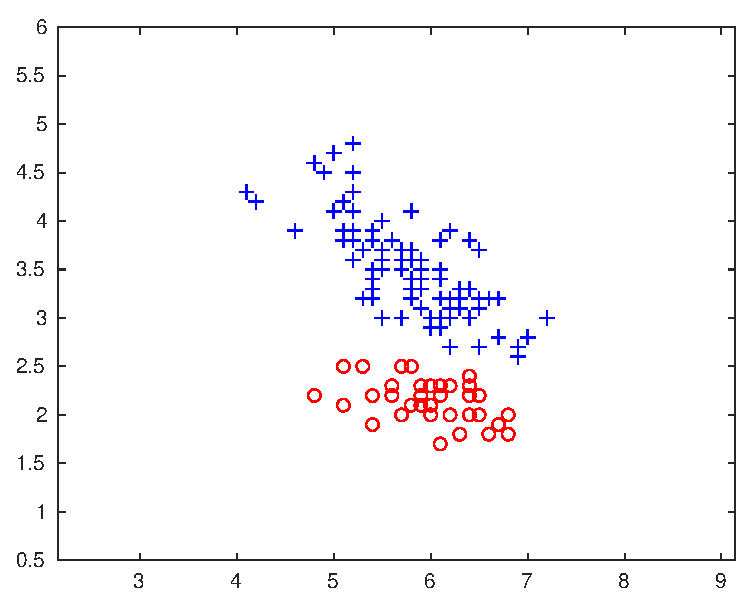
\includegraphics{plot1}
		\caption{The dataset was labeled into two groups indicated by (+) and ($\circ$) in this figure.}
	\end{figure}
	\begin{figure}[H]
		\centering
		\includegraphics{plot2}
		\caption{Data set after binary classification by kmeans algorithm. The two generated mean data points are indicated by the large black (*) symbols.}
	\end{figure}
	\begin{table}[H]
		\caption{Data Misclassified by kmeans}
		\centering
		\begin{tabular}{ c | c | c }
			\hline
			\hline	
			Data Point & Predicted Label & Actual Label\\
			\hline
			(6, 2.9) & -1 & 1\\
			(7.2, 3) & -1 & 1\\
			(6.3, 3.1) & -1 & 1\\
			(6, 2.9) & -1 & 1\\
			(6, 3) & -1 & 1\\
			(6.6, 3.2) & -1 & 1\\
			(6.1, 2.9) & -1 & 1\\
			(6.3, 3.2) & -1 & 1\\
			(6.7, 3.2) & -1 & 1\\
			(6.2, 2.7) & -1 & 1\\
			(6.2, 3.1) & -1 & 1\\
			(6.6, 3.2) & -1 & 1\\
			(6.1, 3) & -1 & 1\\
			(6.5, 2.7) & -1 & 1\\
			(6.5, 3.1) & -1 & 1\\
			(6.4, 3) & -1 & 1\\
			(6.5, 3.2) & -1 & 1\\
			(6.2, 3.1) & -1 & 1\\
			(6.2, 3) & -1 & 1\\
			(7, 2.8) & -1 & 1\\
			(6.9, 2.6) & -1 & 1\\
			(6.7, 2.8) & -1 & 1\\
			(6.9, 2.7) & -1 & 1\\
			\hline
		\end{tabular}
	\end{table}
	\begin{figure}[H]
		\centering
		\includegraphics{plot4}
		\caption{Data seperated by hyperplane generated by perceptron algorithm.}
	\end{figure}
	\begin{figure}[H]
		\centering
		\includegraphics{plot5}
		\caption{Data seperated by hyperplane generated by SVM algorithm.}
	\end{figure}
	\begin{figure}[H]
		\centering
		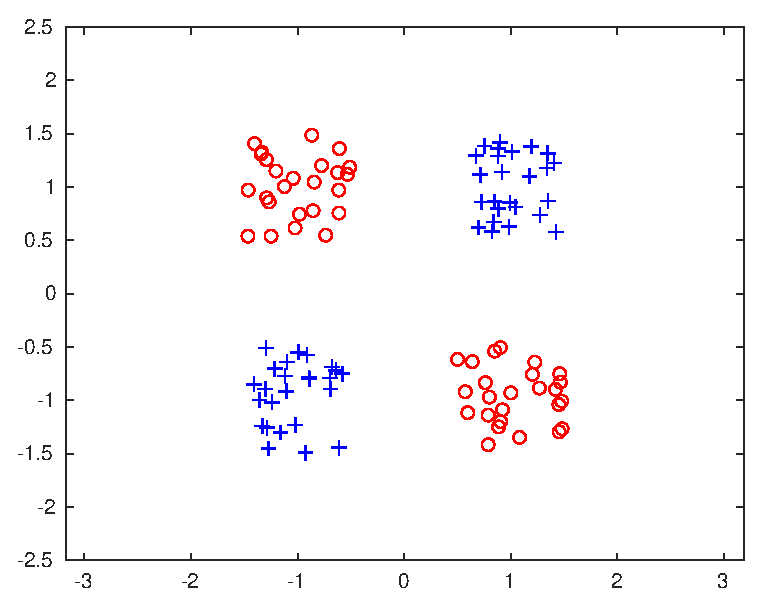
\includegraphics{plot6}
		\caption{Linearly non-seperable dataset before projection. There is no way to divide this data with a hyperplane such that the blue crosses and red circles are on opposite sides.}
	\end{figure}
	\begin{figure}[H]
		\centering
		\includegraphics{plot7}
		\caption{Second dataset after projection and linear seperation. Projection was done by setting the third coordinate of each data point equal to the product of the first two coordinates.}
	\end{figure}
	
	\section*{Discussion}
	The kmeans algorithm generated two classifications with reasonable accuracy, but there were 23 misclassifications (Table 1). This was almost certainly caused by the closeness of the two data classes, as can be seen in (Figure 1). This is consistent with the known fault in kmeans algorithm, where data points closer in proximity to the opposite mean point tend to be misclassified. Note that all misclassified points belonged to the same class, -1 (Table 1). This is probably caused by the data in class -1 being more spread out than the data in class +1 (Figure 1). The perceptron algorithm did create a valid hyperplane that seperates the two classes in such a way that no data point is misclassified (Figure 3), however the line passes very close to several data points in each class, which is consistent with previously verified flaws of the perceptron algorithm. The application of the SVM algorithm generated a hyperplane with the highest possible margin between classes, which is what was expected (Figure 5). The projection of the second data set into the third dimension allowed us to linearly seperate the data (Figure 6), which is what we expected to be able to do. Overall, all methods of binary classification performed as expected and exhibited every flaw that we expected them to. 
	\section*{References}
	1. Ellis, Randy. CISC271 Class 28, Classification - K-Means Clustering [Internet]. 2019-03 [cited 2019-04-11]. \url{https://onq.queensu.ca/content/enforced/260955-CISC271/Notes/Class28.pdf}\\\\
	2. Ellis, Randy. CISC271 Class 30, Classification - Perceptron Algorithm [Internet]. 2019-03 [cited 2019-04-11]. \url{https://onq.queensu.ca/content/enforced/260955-CISC271/Notes/Class30.pdf}\\\\
	3. Ellis, Randy. CISC271 Class 31, Classification - Support Vectors [Internet]. 2019-03 [cited 2019-04-11]. \url{https://onq.queensu.ca/content/enforced/260955-CISC271/Notes/Class31.pdf}\\\\
	4. Ellis, Randy. CISC271 Class 32, Classification - Non-Linear Seperation [Internet]. 2019-03 [cited 2019-04-11]. \url{https://onq.queensu.ca/content/enforced/260955-CISC271/Notes/Class32.pdf}\\\\
\end{document}